\chapter{Vorlesung}

\section{Kanalcodierung}
Der Begriff \emph{Kanalcodierung} bezeichnet das Verfahren, digitale Daten für die Übertragung über gestörte Übertragungskanäle durch das Hinzufügen von Redundanz vor Übertragungsfehlern zu schützen. \cite{WikiKanalCodierung}

\subsection{Datenübertragung und Fehlersicherung}
\begin{figure}
%	\centering
	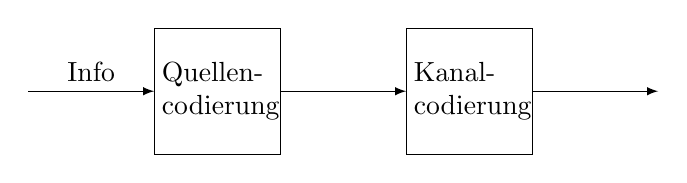
\begin{tikzpicture}[scale =0.8]
		\draw [-latex] (0,1) -- (2,1) node[midway, above] {Info};
		\draw (2,0) rectangle (4,2) node[text width = 40, midway]{Quellen- codierung};
		\draw [-latex] (4,1) -- (6,1);
		\draw (6,0) rectangle (8,2) node[text width = 40, midway]{Kanal- codierung};
		\draw [-latex] (8,1) -- (10,1);
	\end{tikzpicture}	
	\caption{Datenübertragung}
	\label{fig:SchemaDaten}
\end{figure}